\documentclass[onecolumn, draftclsnofoot,10pt, compsoc]{IEEEtran}
\hbadness=1000 % suppress warnings
\usepackage{graphicx}
\usepackage{url}
\usepackage{setspace}
\usepackage{hyperref}
\usepackage{listings}
\usepackage{cite}
\usepackage{geometry}
\usepackage{pdfpages}
\usepackage{longtable}
\include{pygments.tex}

\geometry{textheight=9.5in, textwidth=7in}

% 1. Fill in these details
\def \CapstoneTeamName{		Aerolyzer}
\def \CapstoneTeamNumber{		19}
\def \GroupMemberOne{			Daniel Ross}
\def \GroupMemberTwo{			Logan Wingard}
\def \CapstoneProjectName{		Aerolyzer}
\def \CapstoneSponsorPerson{		Kim Whitehall}


% 2. Uncomment the appropriate line below so that the document type works
\def \DocType{		%Problem Statement
	%Requirements Document
	%Technology Review
	%Design Document
	%Progress Report
	Final Report
}

\newcommand{\NameSigPair}[1]{\par
	\makebox[2.75in][r]{#1} \hfil 	\makebox[3.25in]{\makebox[2.25in]{\hrulefill} \hfill		\makebox[.75in]{\hrulefill}}
	\par\vspace{-12pt} \textit{\tiny\noindent
		\makebox[2.75in]{} \hfil		\makebox[3.25in]{\makebox[2.25in][r]{Signature} \hfill	\makebox[.75in][r]{Date}}}}
% 3. If the document is not to be signed, uncomment the RENEWcommand below
\renewcommand{\NameSigPair}[1]{#1}

%%%%%%%%%%%%%%%%%%%%%%%%%%%%%%%%%%%%%%%
\graphicspath{{images/}}
\begin{document}
	\begin{titlepage}
		\pagenumbering{gobble}
		\begin{singlespace}
			\centering
			
\includegraphics[height=4cm,natwidth=345,natheight=435]{images/coe_v_spot1.png}
			\hfill 
			% 4. If you have a logo, use this includegraphics command to put it on the coversheet.
			%\includegraphics[height=4cm]{CompanyLogo}   
			\par\vspace{.2in}
			\centering
			\scshape{
				\huge CS Capstone \DocType \par
				{\large\today}\par
				\vspace{.5in}
				\textbf{\Huge\CapstoneProjectName}\par
				\vfill
				{\large Prepared for}\par
				{\Large\NameSigPair{\CapstoneSponsorPerson}\par}
				{\large Prepared by }\par
				Group\CapstoneTeamNumber\par
				% 5. comment out the line below this one if you do not wish to name your team
				\CapstoneTeamName\par 
				\vspace{5pt}
				{\large
					\NameSigPair{\GroupMemberOne}\par
					\NameSigPair{\GroupMemberTwo}\par
				}
				\vspace{20pt}
			}
			\begin{abstract}  
				The Aerolyzer Project aims to deliver a new source of air quality and weather information through leveraging existing weather data and image analysis algorithms.
				When complete, this open-source project shall feature a Python library that uses image classification and third-party weather APIs, displayed with an intuitive web-based user interface.
				This document outlines the software design descriptions for the Aerolyzer Library. 
			\end{abstract}     
		\end{singlespace}
	\end{titlepage}

\tableofcontents
\clearpage

\begin{singlespace}

	\section{Introduction}
		todo
	\section{Requirements Document}
		
\includepdf[pages=-]{pdfs/require.pdf}
	\section{Design Document}
		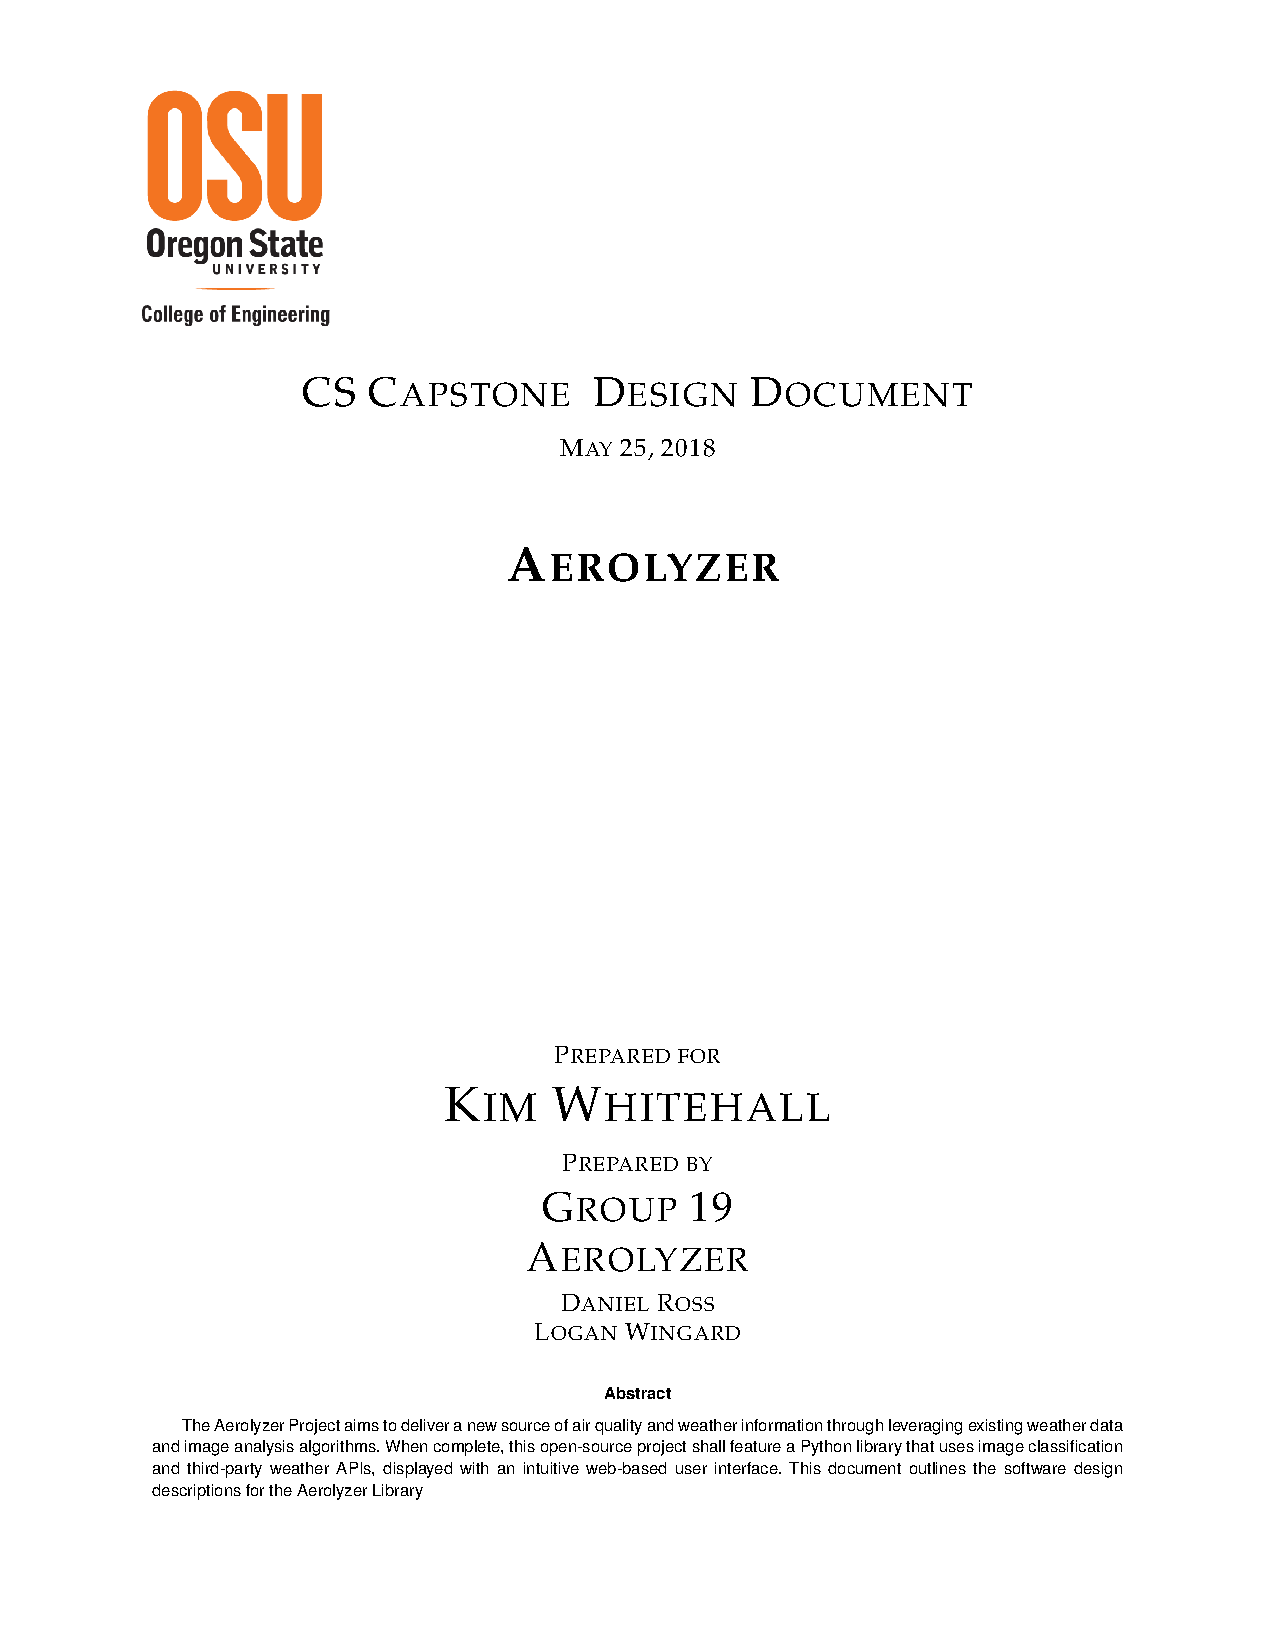
\includepdf[pages=-]{pdfs/design.pdf}
	\section{Tech Review}
		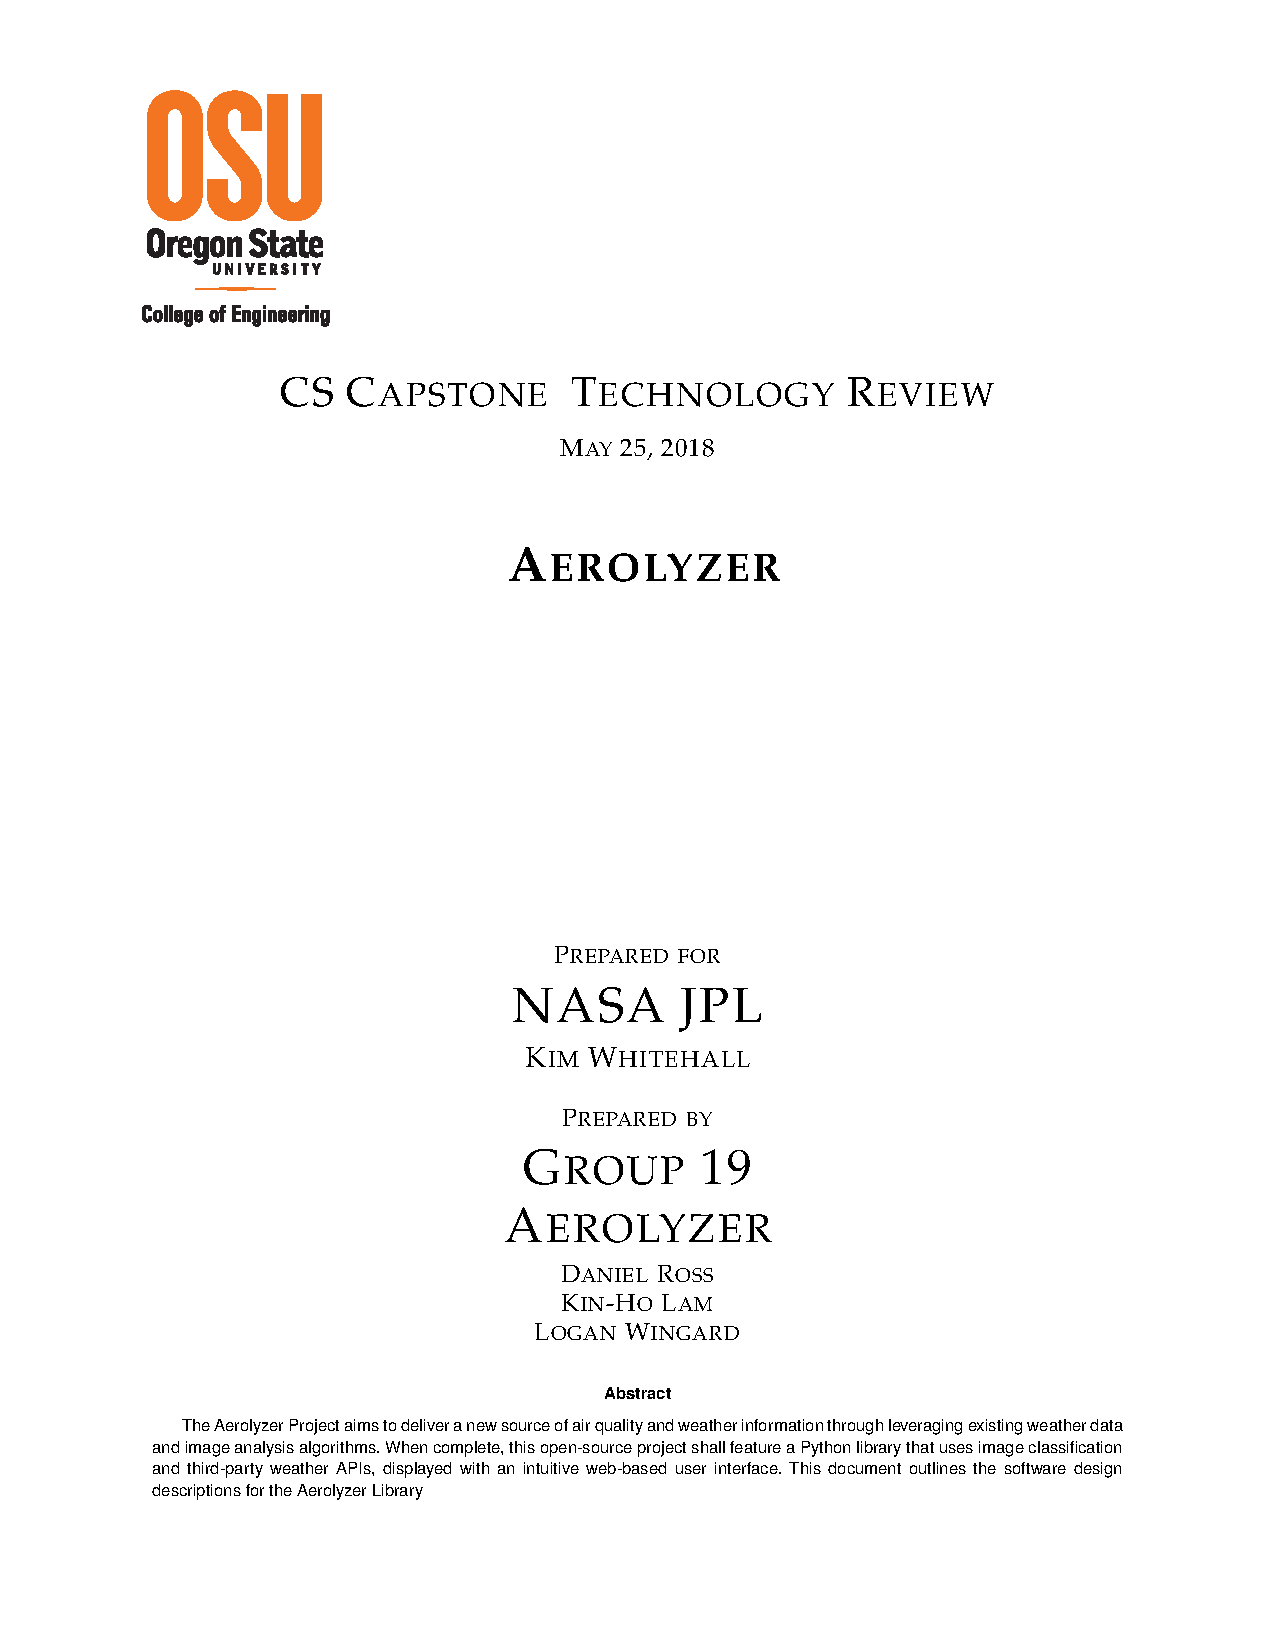
\includepdf[pages=-]{pdfs/tech.pdf}
	\section{Blog Posts}
		\subsection{Daniel Ross}
			todo
		\subsection{Logan Wingard}
			todo
	\section{Poster}
		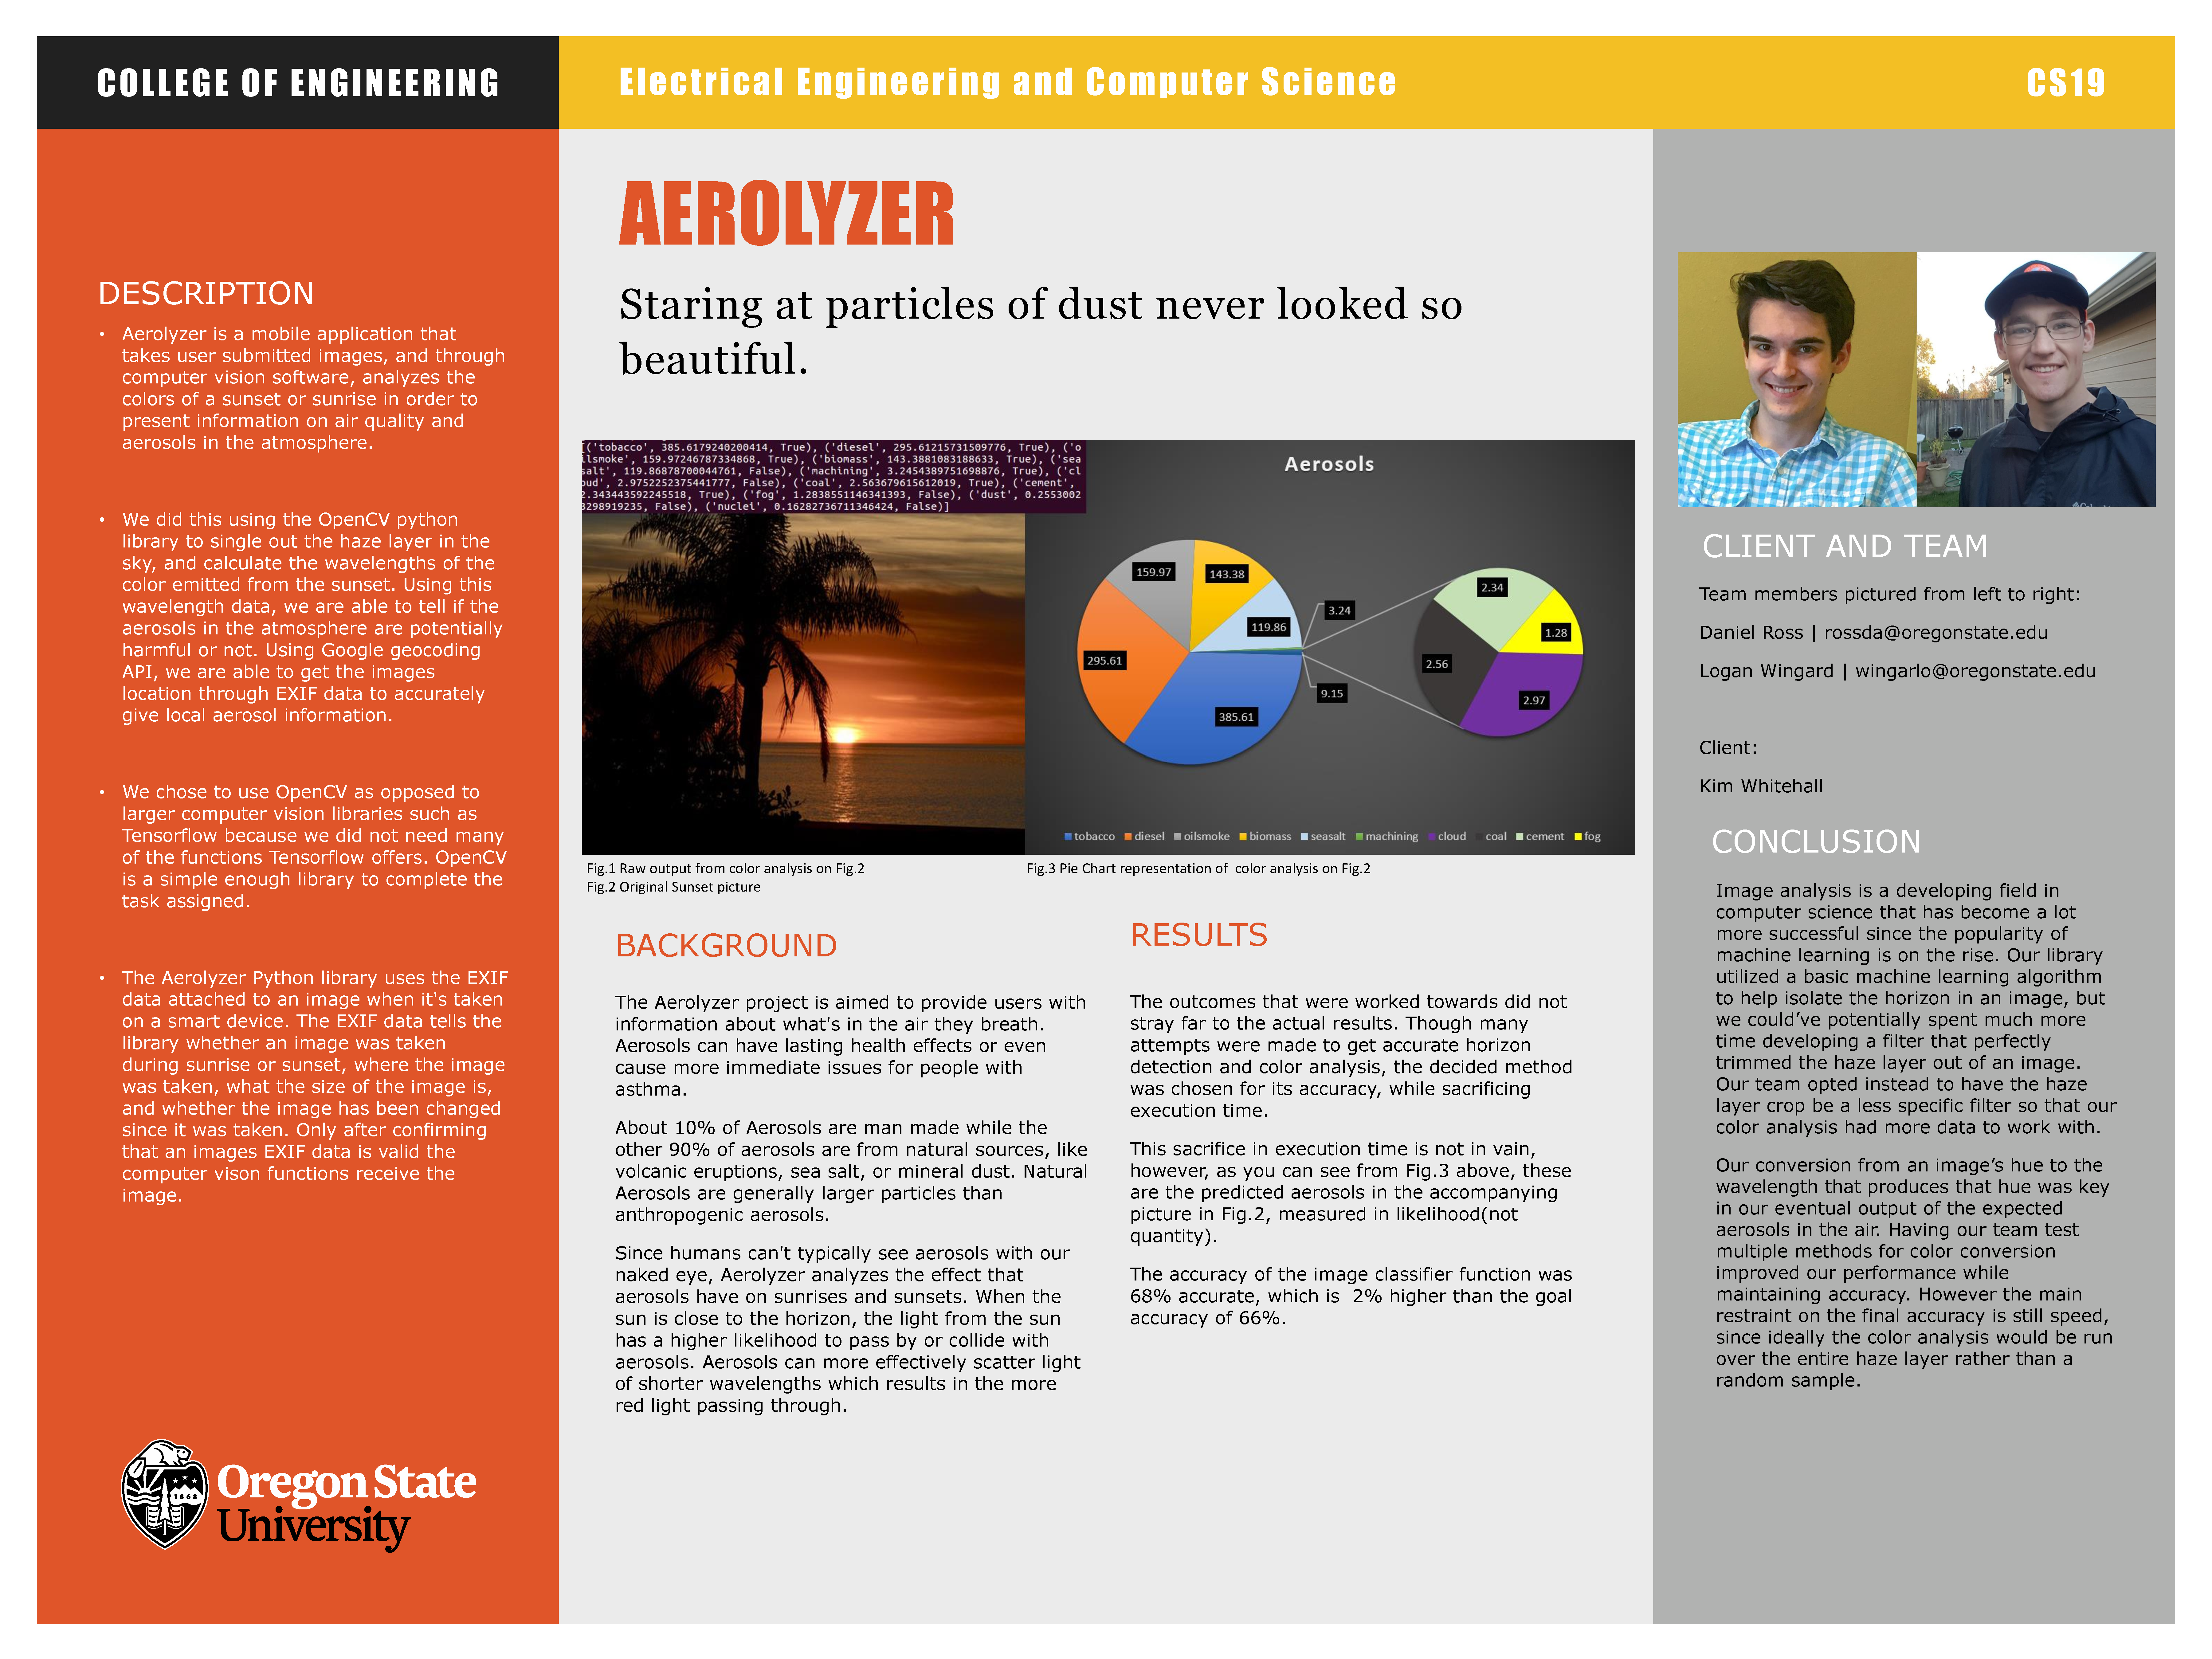
\includepdf[pages=-]{pdfs/poster.pdf}
	\section{Project Documentations}
		todo
	\section{Recommended Resources for Learning More}
		todo
	\section{Conclusion}
		todo \cite{neural}
	\section{Appendix}
		todo
\end{singlespace}
\clearpage
\bibliographystyle{IEEEtran}
\bibliography{ref}
\end{document}
